\documentclass{article}
\usepackage{graphicx} % Required for inserting images
\usepackage[legalpaper, top=1.5cm]{geometry}
\usepackage[backend=biber, style=numeric]{biblatex}
\usepackage{hyperref}


% You can change 'plain' to 'ieeetr', 'alpha', 'apalike', etc.
\bibliography{references} % Put your filename here, WITHOUT the .bib extension

\title{Documentation: Smart Lifevest}
\author{John Louis D. Lagramada}
\date{May 1, 2026}

\hypersetup{
    colorlinks=true,       % False for boxes, true for colored text
    urlcolor=blue,         % Color for external URLs
}

\begin{document}

\maketitle

Please find the codes in the repository provided in this \href{https://github.com/lukasdante/esp32-lifevest-telemetry-2}{Github repository}.

\section{Software}
This section outlines the embedded software architecture governing the Smart Lifevest system. The software is designed around a strictly non-blocking, interrupt-driven paradigm to ensure real-time responsiveness. It handles concurrent tasks including biological signal processing, geolocation parsing, peripheral actuation, and wireless telemetry, operating continuously to bridge the gap between physical sensor data and the external gateway network.
% add network architecture
% add software architecture
\subsection{Lifevest Device}
The Lifevest Device (Edge Transmitter) operates on an ESP32 microcontroller and acts as the primary data acquisition and local processing hub. The firmware is structured around a 3000-millisecond main telemetry loop, punctuated by a high-frequency hardware timer interrupt for precise sensor sampling. This architecture allows the device to function autonomously, evaluating localized threats (such as a spiked heart rate) while maintaining synchronized communication with the gateway.

\subsubsection{Pam-Tompkins Algorithm}
To accurately extract the heart rate from noisy Electrocardiogram (ECG) data, the device implements Smoothed Mode 3 of the Pan-Tompkins algorithm. The system uses an ESP32 hardware timer (\verb|esp_timer|) to sample the analog sensor at exactly 200 Hz, placing the raw 12-bit ADC values into a 1000-sample circular buffer. The signal undergoes several digital signal processing stages within the timer callback:

\begin{itemize}
\item \textbf{Low-Pass Filter}: Attenuates high-frequency muscle noise and powerline interference. The difference equation implemented is:
$$y[n] = 2y[n-1] - y[n-2] + x[n-1] - 2x[n-7] + x[n-13]$$

\item \textbf{High-Pass Filter}: Removes baseline wander. The code implements this using the delayed outputs of the low-pass filter buffer:
$$y[n] = y[n-1] - \frac{x[n-1]}{32} + x[n-17] - x[n-18] + \frac{x[n-33]}{32}$$

\item \textbf{Derivative Filter}: Highlights the QRS complex slopes. The implementation applies a five-point derivative:
$$y[n] = \frac{1}{8} (2x[n-1] + x[n-2] - x[n-4] - 2x[n-5])$$

\item \textbf{Squaring Function}: Makes all data points positive and non-linearly amplifies the higher frequency components of the QRS complex:
$$y[n] = (x[n])^2$$

\item \textbf{Moving Window Integration (MWI)}: Smooths the squared signal to produce a single distinct peak for each heartbeat. The window size ($N$) is set to 30 samples:
$$y[n] = \frac{1}{N} \sum_{i=0}^{N-1} x[n-i]$$

\item \textbf{Peak Detection \& QRS Validation}: The algorithm waits for an initialization period to establish a dynamic baseline threshold (SPKI and NPKI). Detected peaks are validated against a QRS width constraint (between 0.08 and 0.20 seconds) and a refractory period (0.3 seconds) to prevent double-counting the T-wave.

\item \textbf{Smoothing}: The final Beats Per Minute (BPM) is derived from the average of up to 8 recent R-R intervals. To prevent erratic jumping, the BPM change is rate-limited to a maximum delta of 1.0 BPM per second.
\end{itemize}

\subsubsection{Location Tracking}
Geographical coordinate parsing is handled by the TinyGPSPlus library. The ESP32 communicates with a GPS module over a dedicated hardware serial connection \verb|HardwareSerial gpsSerial(2)| at a baud rate of 9600.
\begin{itemize}
    \item In the main loop, \verb|gps.encode()| continuously parses incoming NMEA sentences without blocking execution. 
    \item The software abstracts the retrieval of coordinates into a \verb|getActiveGps()| helper function. If the GPS lock is valid, it extracts the floating-point latitude and longitude. For the first GPS lock, the buzzer and LED actuates for three (3) short bursts.

\end{itemize}

\subsubsection{Automatic LoRa \& GPS Reconnection}
The system relies on fault-tolerant loops to maintain connectivity:

\begin{itemize}
    \item \textbf{LoRa Initialization}: The \verb|attemptLoraConnection()| routine actively toggles the physical reset pin (\verb|RST|) of the LoRa module to ensure a clean boot state before attempting to initialize communication at 433 MHz. If initialization fails, the thread traps into a non-blocking 1000-millisecond delay loop, attempting to re-establish the SPI connection indefinitely until LoRa connects.

    \item \textbf{GPS Reconnection \& Status Tracking}: The firmware records the system timestamp every time a byte is read from the GPS module. The \verb|updateGPS()| routine actively compares the current time against the last time the GPS received data. If the data age exceeds 5000 milliseconds, the system flags the GPS as inactive, effectively invalidating stale location data until the satellite fix is reacquired.
\end{itemize}


\subsubsection{Emergency Actuation}
The lifevest utilizes Pulse Width Modulation (PWM) to drive an emergency LED and a buzzer, allowing for varied intensity if needed.

\begin{itemize}
    
\item Both peripherals are attached to PWM channels operating at a frequency of 2000 Hz with an 8-bit resolution, driven at a 50\% duty cycle (128 out of 255).

\item Actuation is handled asynchronously via \verb|startAsyncSignal()|, which tracks elapsed time against a target duration to toggle the pins on and off.

\item Actuation can be triggered manually via a LoRa command, or automatically if it is enabled and the Pan-Tompkins algorithm reports a heart rate exceeding the heart rate threshold.

\end{itemize}

\subsubsection{Non-volatile Settings}
To ensure configuration persistence across reboots and battery changes, the firmware utilizes the ESP32's internal flash memory via the Preferences library.

\begin{itemize}
\item Upon boot, the device mounts a namespace titled "vest-settings" and loads variables into RAM, falling back to safe defaults if no prior settings exist.

\item The stored settings dictate the system's core behavior, including automatic signaling rules, heart rate thresholds, actuation duration, and toggles for the LED and buzzer.

\item When the device receives a specific LoRa payload (Command Code 2), it instantly updates these live variables and overwrites the Non-Volatile Storage (NVS), ensuring the new parameters remain intact permanently.
\end{itemize}

\subsection{Ground Receiver Station}
The Ground Receiver Station, acting as a gateway, is the critical bridge between the localized, low-power wearable device network and the wider internet. Running on a secondary ESP32 microcontroller, it listens for incoming radio signals from the lifevest and forwards that telemetry to a centralized web server. Its software architecture is built around robust network management, ensuring continuous operation even in fluctuating network conditions.

\subsubsection{Automatic LoRa \& WiFi Reconnection}
To maintain a continuous flow of data, the gateway features independent, automated recovery mechanisms for both its radio and internet connections:
\begin{itemize}
\item \textbf{LoRa Hardware Recovery:} During startup or in the event of a radio module failure, the system actively reboots the physical LoRa chip by toggling its hardware reset pin. It then attempts to initialize communication on the 433 MHz band. If the chip is unresponsive, the system enters a loop, retrying once every second until a successful link is confirmed.
\item \textbf{Non-blocking WiFi Watchdog:} The internet connection is monitored continuously during the system's main operational loop. If the WiFi drops, the system registers the disconnection and triggers a recovery routine. Instead of freezing the entire system while waiting for the router, it attempts to reconnect in the background once every five seconds, allowing the radio module to continue listening for emergency distress signals seamlessly.
\end{itemize}

\subsubsection{HTTPS POST Request}
Whenever the gateway intercepts a valid radio transmission containing the correct authentication password, it immediately translates the binary radio packet into a web-friendly JSON format.
\begin{itemize}
\item The payload constructed includes the device's unique identifier (\verb|vest_id|), the user's current \verb|heart_rate|, geographical coordinates (\verb|latitude| and \verb|longitude|), and critical network health metrics (radio signal strength and noise ratio).
\item This data is securely forwarded to the cloud infrastructure via an HTTPS POST request.
\item The system is designed to gracefully handle network timeouts, dropping the transmission if the server does not respond within 1.5 seconds, ensuring the gateway quickly returns to listening for the next radio pulse.
\end{itemize}

\subsubsection{HTTPS Piggybacking}
To minimize latency and network overhead, the system utilizes a "piggybacking" technique to receive instructions from the web server. Rather than the gateway constantly asking the server if there are new commands, the server attaches any pending instructions directly to its reply after receiving a telemetry update.
\begin{itemize}
\item Upon a successful telemetry upload, the gateway reads the server's response payload and scans it for a command code (\verb|cmd|).
\item If a command code greater than zero is detected, the system understands that the web application wants to update the lifevest's settings or trigger an alarm manually.
\item To parse the incoming data without utilizing heavy, memory-intensive JSON libraries, the gateway uses a custom extraction function that hunts for specific key names (like \verb|hr| for heart rate thresholds or \verb|dur| for signal durations) and pulls out the associated numerical values.
\end{itemize}

\subsubsection{Command Transmission and Acknowledgement}
Once the gateway decodes a piggybacked command from the internet, it must ensure that the physical lifevest actually receives and executes it over the LoRa radio network. It accomplishes this through a reliable delivery and retry loop:
\begin{itemize}
\item \textbf{Transmission and Wait State:} The gateway packages the instructions into a new radio packet, broadcasts it to the edge device, and flags the system as awaiting an acknowledgement (\verb|isAwaitingAck|). It simultaneously records the exact time the command was sent.
\item \textbf{Retry Logic:} If three seconds elapse without a confirmation reply from the lifevest, the gateway assumes the packet was lost in the airwaves and re-transmits the command. It will attempt this up to five times (\verb|retryCount|) before conceding that the vest is unreachable.
\item \textbf{Server Notification:} If the lifevest successfully receives the command and replies with a valid acknowledgement packet, the gateway immediately cancels its retry timer. It then fires a final, brief HTTP POST request back to a dedicated server endpoint to confirm that the instruction was successfully fulfilled.
\end{itemize}

\subsection{Website}
The website serves as the central command and monitoring hub for the Smart Lifevest system. Hosted entirely in the cloud, it is responsible for securely receiving the relayed data from the ground receiver station, permanently storing this information, and serving a live dashboard to both end-users and system administrators.

\subsubsection{Database}
The system's memory is structured as a relational database, designed to efficiently link user profiles with their real-time geographical and biological data.

\begin{itemize}
\item \textbf{Entity Relationship Diagram}: 
\begin{figure}[htbp]
    \centering
    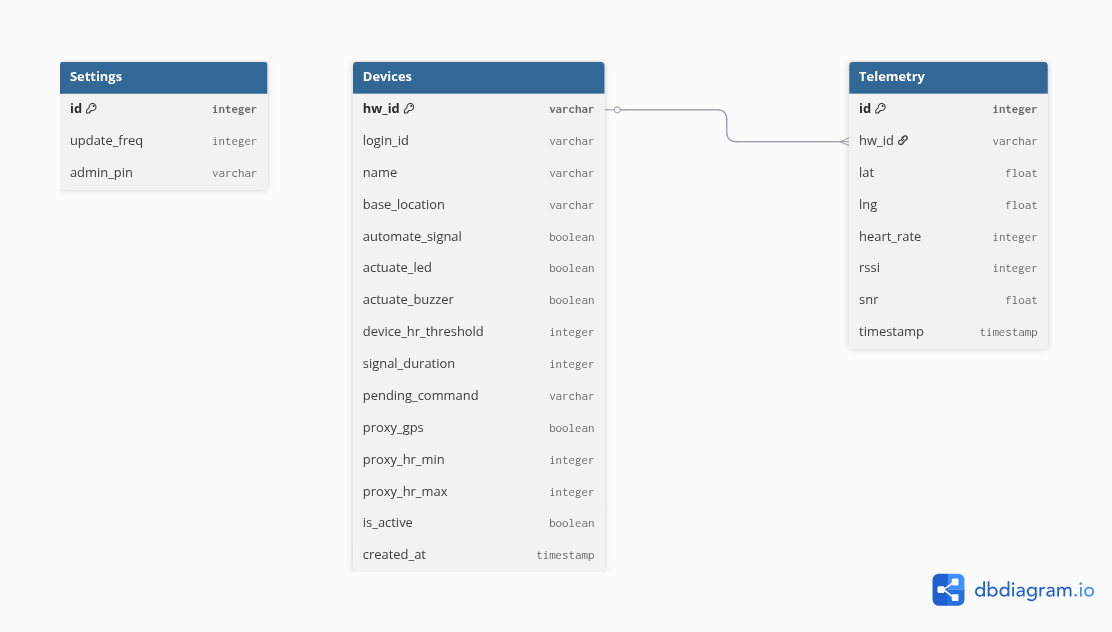
\includegraphics[width=0.8\textwidth]{../erd.png}
    \caption{Entity relationship diagram.}
    \label{fig:my_diagram}
\end{figure}
The database architecture is divided into three primary categories:
\begin{itemize}
\item The \verb|Devices| table acts as the master registry. It bridges the physical hardware identifier (\verb|hw_id|) to a user-facing access code (\verb|login_id|). Beyond identification, it stores the personalized safety parameters for each vest, such as the heartbeat limit (\verb|device_hr_threshold|) and whether the alarms should trigger on their own (\verb|automate_signal|). It also contains a vital \verb|pending_command| queue, which acts as a holding area for instructions waiting to be sent back down to the physical lifevest.
\item The \verb|Telemetry| table serves as the continuous logbook. Every time the lifevest transmits a pulse, a new record is created here containing the user's \verb|heart_rate|, exact GPS coordinates (\verb|lat| and \verb|lng|), radio signal quality, and a precise \verb|timestamp|. This table is strictly tethered to the Devices table; if an administrator deletes a vest from the system, all of its historical tracking data is automatically erased as well.

\item The \verb|Settings| table is a secure, isolated configuration file that holds global variables for the web application, such as the master password (\verb|admin_pin|) required to access the backend dashboard.
\end{itemize}
\item \textbf{Scheduled Telemetry Table Refresh}: 
Because the lifevest transmits data every few seconds, the database could quickly become bloated with millions of location points, slowing down the server and incurring high storage costs. To prevent this, the software includes an automated daily cleanup routine. Operating on a strict schedule (a CRON job set to run at midnight), the server sweeps through the \verb|Telemetry| table and permanently deletes any tracking records that are older than one day. This ensures the database remains lightweight and focused only on the user's most recent activity.
\end{itemize}

\subsubsection{Cloud Deployment}To guarantee that the monitoring system remains online during emergencies without the need for manual server maintenance, the backend is deployed entirely on a "serverless" cloud infrastructure.

\begin{itemize}

\item \textbf{Cloudflare Domains}: The cloud provider manages the domain routing, ensuring that all data—whether it is a telemetry upload from the ground station or a user checking their dashboard on a smartphone—is transmitted over a secure, encrypted HTTPS connection. This prevents sensitive geographical and heart rate data from being intercepted over public networks.

\item \textbf{Cloudflare Workers}: Instead of a traditional server computer that runs constantly, the application's core logic runs on Cloudflare Workers using the Hono web framework. In this environment, the server code effectively "sleeps" until an event occurs—such as a user loading the website or the receiver station sending a \verb|POST| request containing new data. Once triggered, the worker instantly wakes up, processes the data, and shuts back down. This architecture also securely manages access, utilizing an \verb|adminAuth| checkpoint to intercept requests and verify the administrator's PIN before allowing any changes to the system.

\item \textbf{Cloudflare D1}: 
This is the cloud-native SQL database system that houses the tables mentioned above. Bound directly to the serverless Worker under the name \verb|lifevest-db|, it allows the application to instantly read and write emergency data across a globally distributed network without the delays typically associated with connecting to traditional, centralized database servers.
\end{itemize}

\subsubsection{Login}
\begin{itemize}
\item \textbf{User}: The user login interface (\verb|index.html|) provides a simple, direct entry point for tracking a specific lifevest. Users input a unique, secure "session ID" (e.g., VEST-892A) into the \verb|#lifevestId| field. Upon submission, the frontend Javascript intercepts the request and verifies the ID against the backend database using the \verb|/api/live/:login_id| endpoint. If the ID is valid and active, the user is seamlessly routed to the tracking dashboard.
\item \textbf{Admin}: The administrative interface (\verb|admin.html|) acts as the control center for the entire fleet. Access is restricted via a secure PIN overlay (\verb|#adminAuthOverlay|). The entered PIN is verified against the backend settings database. Once authenticated, administrators can view the real-time online status of all registered hardware, assign new lifevests to login session IDs, modify global polling frequencies, and change the admin password.
\end{itemize}

\subsubsection{Dashboard}
The Dashboard is the primary graphical user interface for the system, accessible via a web browser on a smartphone or computer. It translates raw telemetry data from the database into an intuitive, real-time tracking and control center for the user.  \begin{itemize}
\item \textbf{Settings}: Users can customize the behavior of the specific lifevest they are tracking via a dedicated configuration menu.
\begin{itemize}
\item This menu allows the adjustment of critical parameters, including the \verb|hr_threshold| (the beats-per-minute limit that triggers an alarm), the \verb|signal_duration| for the emergency peripherals, and manual toggles to enable or disable the LED and buzzer independently.
\item When saved, the web interface packages these settings and queues them in the database to be "piggybacked" to the physical lifevest during its next transmission cycle.
\end{itemize} 
\item \textbf{Geolocation Tracking and Waypoint}: The dashboard utilizes an interactive digital map to visualize the exact geographical coordinates of both the smartphone (the viewer) and the lifevest (the wearer). 
\begin{itemize}
    \item A dynamically drawn dashed line visually connects the two markers on the screen.
    \item To enhance situational awareness, the interface features a synchronized radar animation; it calculates the physical distance between the two points and precisely delays a flashing animation on the wearer's icon so that it illuminates exactly when the viewer's expanding radar wave "hits" it on the screen.
\end{itemize}

\item \textbf{Phone Navigational Mode}: For active search-and-rescue scenarios, the user can toggle a specialized navigation mode. 
\begin{itemize}
    \item When activated, the web application requests permission to access the smartphone's internal compass (magnetometer). 
    \item The software then locks the map camera to the user's location and actively rotates the entire map container inversely to the phone's physical heading. This ensures the digital map always aligns with the real world, similar to dedicated turn-by-turn GPS applications.
\end{itemize}

\item \textbf{Heart Rate and Distance Display}: Real-time vital signs and spatial data are persistently displayed at the bottom of the screen. 
\begin{itemize}
    \item The system calculates the exact distance in meters between the phone's GPS and the lifevest's GPS.
    \item The heart rate monitor constantly compares the live BPM against the user-defined threshold. If the threshold is exceeded, the interface automatically triggers a "Distress Mode," turning the text red, updating the status label to "IN DISTRESS," and applying a red visual vignette overlay across the entire screen to immediately alert the viewer.
\end{itemize}

\item \textbf{Lifevest Status}: A prominent status badge informs the user of the system's overall health and connectivity. 
\begin{itemize}
    \item This is determined by evaluating the timestamp of the most recent data packet. 
    \item If data was received within the last 30 seconds, it displays as "LIVE". If the delay exceeds 30 seconds, it degrades to "WAITING," and if a full 60 seconds pass without a signal, the system officially marks the lifevest as "OFFLINE".
\end{itemize}

\item \textbf{Connection Strength}: To help users understand the reliability of the radio link, the dashboard includes a standard four-bar cellular-style signal indicator. 
\begin{itemize}
    \item The system dynamically fills these bars based on the Received Signal Strength Indicator (RSSI) of the LoRa packets. For example, an RSSI stronger than -95 dBm grants all four bars, while a signal dropping below -115 dBm reduces it to two. 
    \item If the status degrades to "OFFLINE," the bars are dimmed and a red "X" overlay is dynamically generated to clearly communicate the communication loss.
\end{itemize}

\item \textbf{Signaling Activation}: A central manual override button allows the user to immediately trigger the lifevest's emergency LED and buzzer, regardless of the wearer's heart rate. 
\begin{itemize}
    \item Pressing this button queues an actuation command in the database. 
    \item The button features "Smart ACK Logic," changing its color and text to provide real-time feedback on the radio transmission state. It turns green to indicate the command is queued for the next ping, changes to yellow (displaying "Waiting for Vest ACK...") while the radio gateway transmits it, and returns to its default blue state only when the physical lifevest confirms execution.
\end{itemize}
\end{itemize}

\subsubsection{Admin Page}
The Admin Page serves as the centralized command center for the organization deploying the Smart Lifevests, offering high-level control over the entire network of devices. After successfully bypassing the security overlay with the correct password, administrators are presented with a real-time overview of the active fleet and a suite of management tools.
\begin{itemize}
\item \textbf{Adding, Removing, Modifying Lifevests}: The platform includes a robust fleet management system to handle the physical lifecycle of the hardware:
\begin{itemize}
\item \textbf{Adding}: Administrators can easily register new lifevests into the database by entering the device's physical hardware ID, assigning it a user-friendly name, logging its physical base location, and giving it an initial session ID for a user to log into.
\item \textbf{Modifying}: To accommodate maintenance, the system supports seamless hardware swapping. If a physical vest needs to be replaced, an administrator can edit the device profile and swap the old hardware ID for a new one. The backend software safely migrates all previous tracking history to the new hardware ID so the continuity of the data is never broken.
\item \textbf{Removing}: If a device is permanently retired, it can be deleted from the system. Because deleting a device also permanently erases all of its historical tracking data, the interface triggers a severe visual warning requiring explicit confirmation before the action is executed. Once authorized, both the device profile and its telemetry logs are purged from the database.
\end{itemize}
\item \textbf{Global Settings}: Administrators have the authority to alter overarching parameters that dictate how the web server and the dashboards behave.
\begin{itemize}
    \item \textbf{Update Frequency}: This setting determines the polling rate of the system—specifically, how often (in milliseconds) the user dashboards refresh to pull the latest GPS and heart rate data from the database. Adjusting this allows administrators to balance real-time tracking responsiveness against server load.
    \item \textbf{Security Management}: The global settings panel also provides the interface for changing the master administrative password (PIN) required to access the control center. When updated, the new security credentials are saved directly to the core database and take effect immediately.
\end{itemize}
\end{itemize}



\section{Hardware}

\subsection{Lifevest Device}
% add circuit diagram
\subsubsection{Wireless Charging}
\subsubsection{Waterproofing}
\subsubsection{Antennas}
\subsubsection{Boost Converters}
\subsubsection{MOSFET Control \& Actuators}
\subsubsection{Sensor and Network Modules}
\subsubsection{Modular Velcro Attachment}

\subsection{Ground Receiver Station}
% add circuit diagram
\subsubsection{LoRa Module}




\nocite{*}
\printbibliography

\end{document}